\chapter{Evaluation}
\label{sec:evaluation}

% 1 hasab + 1 abra helyed van, helytakarekosan irj, keruld az itemize-okat

We implemented \incqueryD{} as an initial prototype to evaluate the feasibility of the approach, and to experiment with various optimization possibilities. As the storage, we used the popular graph database Neo4j \cite{neo4j} featuring automatic indexes and two core query technologies (Gremlin and Cypher) that were used as a low-level model access interface by our middleware layer. % TODO middleware: blueprints, but custom implementation because\ldots
The prototype of the distributed middleware and Rete network were implemented in Java using Akka~\cite{akka}, the Scala-based toolkit for building applications based on the Actor model, since it is well-suited for asynchronous applications. The communication protocol was built on top of Akka's built-in serialization support.


%TODO mit merunk? model manipulacios muveletek es query kiertekeles valaszido
%adott: query def, modell manipulacios szekvencia

% 4 fazisban az alabbiak szerint TODO
%generalt: novekvo meretu modellek (hogyan generaltuk, mi a query-k eredmenyhalmaz meretenek viszonya a modellhez?, 

%mi az elosztott modell sajatossaga/limitacioja (nincsenek keresztelek))

%mert: lekerdezesek, ill. manip. tranzakcio lefutasi ideje

\section{Benchmark scenario}

\label{benchmark}
In order to measure the efficiency of model queries and manipulation operations over the distributed architecture, we designed a benchmark to measure tool response times in a well-formedness validation use case. The benchmark transaction sequence consists of four phases: (i) during the $load$ phase, the serialization of the model is loaded into the database; (ii) a test query (\autoref{fig:patterndef}) is executed ($check_0$); finally, in a cycle consisting of several repetitions, some elements are programmatically modified ($edit_i$) and the test query is re-evaluated ($check_i$). We ran the benchmark on pseudo-randomly generated instance models of growing size, each model containing about twice as many elements (vertices and edges) as the previous one and having a regular fan-out structure. As the current version of Neo4j does not have built-in support for graph sharding, the benchmark uses a manually sharded strategy where each shard contains a disjoint partition of the model.


%TODO referencia leirasa (miert az, ami?)
% We implemented two approaches
% on top of Neo4j.
% Non-incremental: uses only Cypher for the pattern matching. 
%   Beside Neo4j's indexes, no additonal data structures are built.

% TODO sajat implementacio leirasa (manualis allokacio)

% Incremental: builds a distributed Rete network to support incremental pattern matching, and 
%     maintains both the databases and the Rete net upon modification. 
%     Only uses Cypher to retrieve the graph nodes for the type indexers of the Rete net. 

% For the incremental query, we manually created the Rete network and 
% generated random instance models of different sizes to benchmark the query's execution time.

\label{benchmark_environment}
\section{Evaluation aspects and benchmark environment}

To compare the performance characteristics of \incqueryD{} to a traditional case, we defined two scenarios. The \textit{batch} scenario uses only Neo4j to manage models and evaluate the queries in a parallelized way (depicted as \textcircled{1} in \autoref{fig:architecture}). This serves as a baseline for the \textit{incremental} scenario, which uses \incqueryD{} (shown as \textcircled{2} in \autoref{fig:architecture}). For these initial experiments, the layout and allocation of the Rete network was determined manually. As the testbed, we deployed our system to a private cloud consisting of 4 virtual machines on separate host computers. Each virtual machine used dual 2.5 GHz Intel Xeon L5420 CPUs with 16 GBs of RAM, running on Ubuntu 12.10 64 bit with Neo4j 1.8 and Akka 2.1.2. More details are available at \url{http://incquery.net/publications/trainbenchmark}.

\begin{figure}
\begin{center}
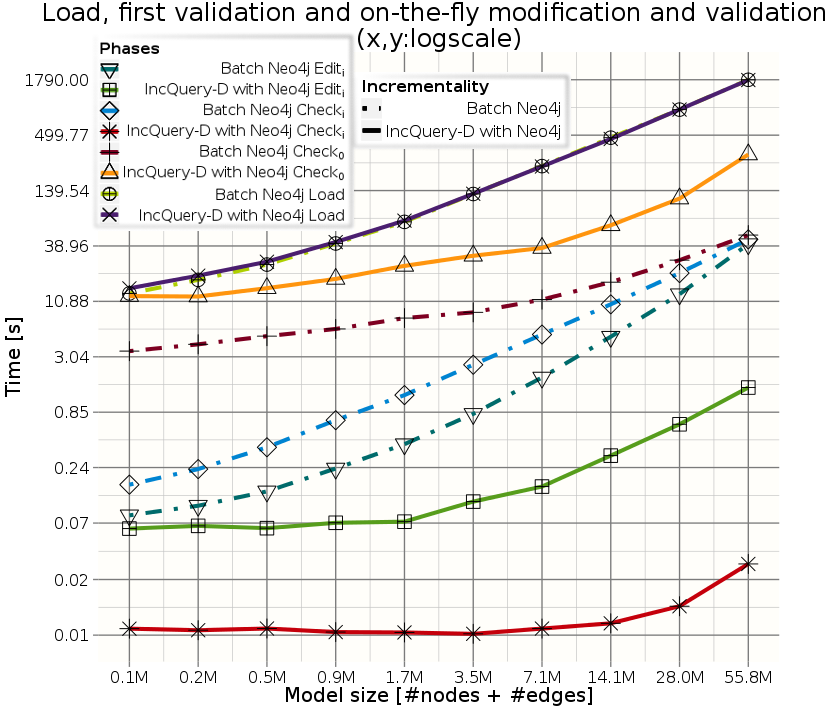
\includegraphics[width=\columnwidth]{figures/All_RouteSensor}
\caption{Benchmark results}
\label{fig:benchmark}
\end{center}
\end{figure}

\section{Results}
\label{benchmark_results}\label{analysis}

The measurement results of our experiments are shown in \autoref{fig:benchmark} (aggregated from several complete sets to filter transient effects). As expected, the $load$ phase take about the same time for both scenarios, and \incqueryD{} is about half an order of magnitude slower when evaluating the query at first (\textit{check 0} phase) due to the Rete construction overhead. However, \incqueryD{} is several orders of magnitude faster during the $edit_i - check_i$ cycles, making on-the-fly query (re)evaluation feasible even for models larger than 50 million elements. Once initialized, \incqueryD{} scales linearly, since query response times for growing models can be kept low by adding additional computers for hosting Rete nodes.

The Rete implementation is based on the Rete algorithm, originally created by Charles Forgy \cite{Forgy} and improved by Gábor Bergmann \cite{BergmannRete}.

\section{Technologies}

\subsection{Akka}

Akka is a toolkit and runtime for building highly concurrent, distributed, and fault tolerant event-driven applications on the JVM \cite{akka}. In my implementation, the remote nodes run on Akka \textit{microkernels}. The actors are instantiated using the \textit{remote deployment} feature.

\begin{figure}
\begin{center}

\includegraphics[width=6cm]{figures/akka-logo}
\caption{The logo of Akka}
\label{fig:akka-logo}
\end{center}
\end{figure}

The alpha nodes (called \textit{UniquenessEnforcerNodes}) store the edges and their source and destination nodes in their memory.

Currently, these graph elements are retrieved by Cypher (\autoref{lst:cypher-route-routedefinition}).

\begin{lstlisting}[caption=Cypher query to retrieve all \texttt{ROUTE\_ROUTEDEFINITION} edges, label=lst:cypher-route-routedefinition, breaklines=true]
START
    route=node:node_auto_index(type='Route'),
    sensor=node:node_auto_index(type='Sensor')
MATCH (route)-[:ROUTE_ROUTEDEFINITION]->(sensor)
RETURN route.idx AS routeId, sensor.idx AS sensorId;
\end{lstlisting}

\subsection{Google Guava}

The implementation relied heavily on Google Guava library's Collections framework \cite{guava}. The Guava Collection is an extension to Java's Collection framework. We used immutable collections and new type of collections (e.g.\ Multimap).

\subsection{Neo4j Java REST binding}

I used Neo4j in \textit{server mode} and accessed the REST interface with the \texttt{java-rest-binding} library \cite{restbinding}.

\subsection{Apache Maven}

To integrate the technologies, we used Apache Maven \cite{Maven}, an open source build automation system.
